\documentclass[aspectratio=169,11pt]{beamer}
\usetheme{default}
\usecolortheme{default}
\usepackage{amsmath,bm}
\usepackage{graphicx}
\usepackage{booktabs}
\usepackage{tikz}
\usetikzlibrary{arrows.meta,positioning}
\graphicspath{{../figures/}}

% ---- look ----------------------------------------------------------------
\definecolor{ink}{HTML}{1F2937}
\definecolor{accent}{HTML}{5B3FA6}
\definecolor{accent2}{HTML}{2E7D32}
\definecolor{soft}{HTML}{F3F0FA}
\setbeamercolor{normal text}{fg=ink}
\setbeamercolor{structure}{fg=accent}
\setbeamercolor{frametitle}{fg=accent,bg=white}
\setbeamercolor{title}{fg=accent}
\setbeamercolor{block title}{fg=white,bg=accent}
\setbeamercolor{block body}{bg=soft}
\setbeamerfont{frametitle}{size=\Large,series=\bfseries}
\setbeamerfont{title}{size=\LARGE,series=\bfseries}
\setbeamertemplate{navigation symbols}{}
\setbeamertemplate{itemize items}[circle]
\setbeamertemplate{footline}{%
  \hfill\textcolor{gray}{\scriptsize\insertframenumber\,/\,\inserttotalframenumber}\hspace{1em}\vspace{0.6em}}
\setbeamertemplate{frametitle}{\vspace{0.6em}\insertframetitle\par\vspace{-0.2em}%
  \textcolor{accent}{\rule{\textwidth}{0.6pt}}}
\newcommand{\takeaway}[1]{\begin{beamercolorbox}[rounded=true,sep=6pt,wd=\textwidth]{block body}\textbf{#1}\end{beamercolorbox}}

\title{Bayesian-Optimized\\Variational Quantum Circuits}
\subtitle{Teaching a 2-qubit circuit to classify data, without gradients}
\author{Jialun Li \and Juan Vera}
\institute{PHYS 126}
\date{\today}

\begin{document}

% 1 ---------------------------------------------------------------------------
\begin{frame}[plain]
  \vspace{1.5em}
  \titlepage
\end{frame}

% 2 ---------------------------------------------------------------------------
\begin{frame}{The question}
  \vspace{0.5em}
  \begin{center}
    \Large Can a \textbf{tiny quantum circuit} learn to classify data\\
    as well as a \textbf{small neural network}\dots\\[0.6em]
    \textcolor{accent}{\textbf{\dots if we train it without gradients?}}
  \end{center}
  \vspace{1.2em}
  \begin{columns}[T]
    \column{0.48\textwidth}
      \textbf{Why ``without gradients''?}
      \begin{itemize}
        \item Neural nets are trained by following the slope of the error.
        \item On a real quantum computer, that slope is \emph{expensive and noisy} to measure.
        \item So people want optimizers that only need the score, not the slope.
      \end{itemize}
    \column{0.48\textwidth}
      \textbf{What we did}
      \begin{itemize}
        \item Built a 2-qubit circuit in Qiskit.
        \item Trained it with \textbf{Bayesian optimization}.
        \item Raced it against classical neural networks on the same task.
      \end{itemize}
  \end{columns}
\end{frame}

% 3 ---------------------------------------------------------------------------
\begin{frame}{The task: two moons}
  \begin{columns}[c]
    \column{0.5\textwidth}
      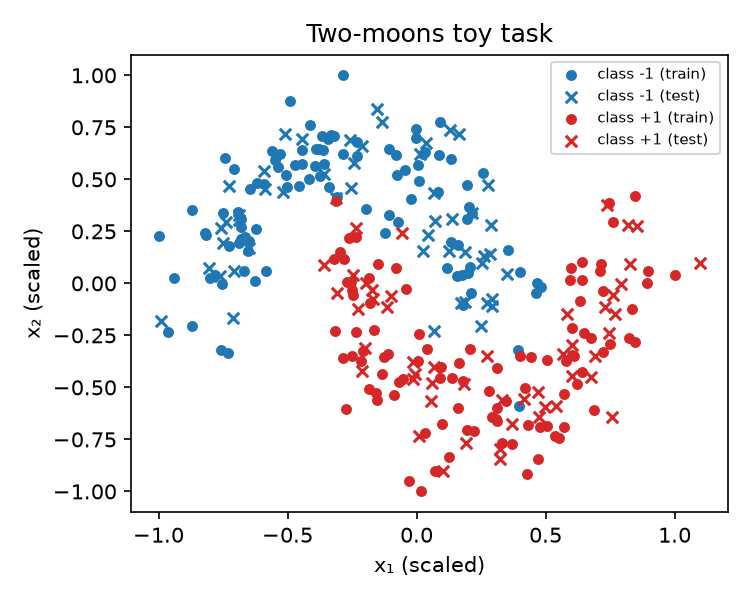
\includegraphics[width=\textwidth]{dataset.png}
    \column{0.47\textwidth}
      \begin{itemize}
        \item 300 points in two interleaved crescents, red and blue.
        \item Goal: given a new point, say which colour it is.
        \item 200 points to learn from, 100 held back to test on.
      \end{itemize}
      \vspace{0.8em}
      \takeaway{No straight line separates them. A straight-line classifier scores 84\,\%. Everything above that needs a \emph{curved} boundary.}
  \end{columns}
\end{frame}

% 4 ---------------------------------------------------------------------------
\begin{frame}{What a quantum classifier is}
  \centering
  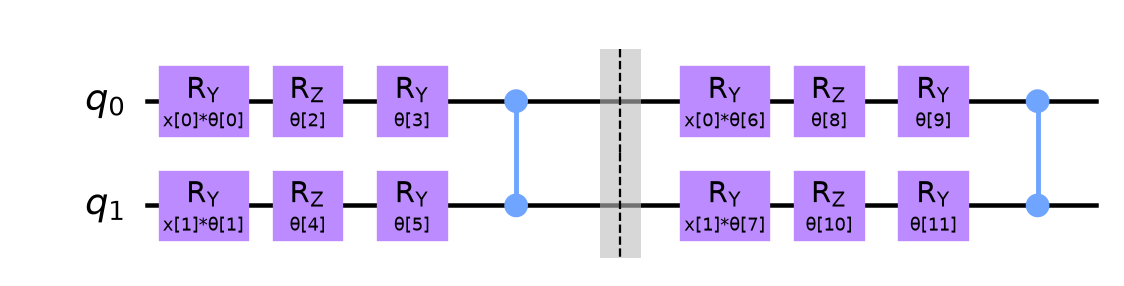
\includegraphics[width=0.72\textwidth]{circuit.png}\\[-0.3em]
  {\footnotesize two of the four layers shown}
  \vspace{0.2em}
  \begin{columns}[T]
    \column{0.55\textwidth}
      \small
      \begin{enumerate}
        \item Rotate each qubit by an angle that depends on the data point $(x_1, x_2)$.
        \item Rotate again by \textbf{trainable} angles $\theta$ (the ``knobs'').
        \item Entangle the two qubits. Repeat four times.
        \item Measure qubit 0.
      \end{enumerate}
    \column{0.42\textwidth}
      \takeaway{Output: a number $f \in [-1, 1]$.\\ $f > 0 \Rightarrow$ red, \quad $f < 0 \Rightarrow$ blue.}
      \vspace{0.5em}
      \small 24 knobs in total. \textbf{Training} = turning the knobs until the sign is right for as many points as possible.
  \end{columns}
\end{frame}

% 5 ---------------------------------------------------------------------------
\begin{frame}{Why we can't just use gradients}
  \small
  \begin{columns}[T]
    \column{0.5\textwidth}
      \textbf{Neural network}
      \begin{itemize}
        \item Backpropagation: one backward pass gives the slope for \emph{every} weight.
        \item Cost $\approx$ one forward pass.
      \end{itemize}
      \vspace{0.6em}
      \textbf{Quantum circuit}
      \begin{itemize}
        \item You can't look inside the state without destroying it, so there is no backward pass.
        \item The slope for one knob costs two extra full runs:
          \[ \frac{\partial f}{\partial \theta} = \tfrac{1}{2}\big[f(\theta + \tfrac{\pi}{2}) - f(\theta - \tfrac{\pi}{2})\big] \]
        \item 24 knobs $\Rightarrow$ \textbf{48 extra runs} per data point per step, each one noisy.
      \end{itemize}
    \column{0.46\textwidth}
      \vspace{1.2em}
      \begin{center}
      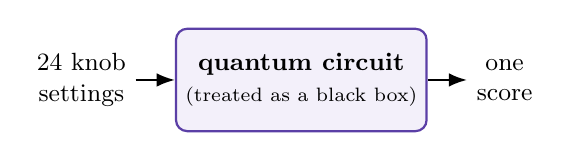
\begin{tikzpicture}[node distance=5mm, >=Latex, font=\small]
        \node[draw=accent, thick, rounded corners, fill=soft, minimum width=2.9cm, minimum height=1.3cm, align=center] (box) {\textbf{quantum circuit}\\ \scriptsize (treated as a black box)};
        \node[left=of box, align=center] (in) {24 knob\\settings};
        \node[right=of box, align=center] (out) {one\\score};
        \draw[->, thick] (in) -- (box);
        \draw[->, thick] (box) -- (out);
      \end{tikzpicture}
      \end{center}
      \vspace{0.6em}
      \takeaway{So we treat it as a black box: knobs in, score out. We need an optimizer that works from scores alone.}
  \end{columns}
\end{frame}

% 6 ---------------------------------------------------------------------------
\begin{frame}{Bayesian optimization in plain words}
  \begin{columns}[c]
    \column{0.5\textwidth}
      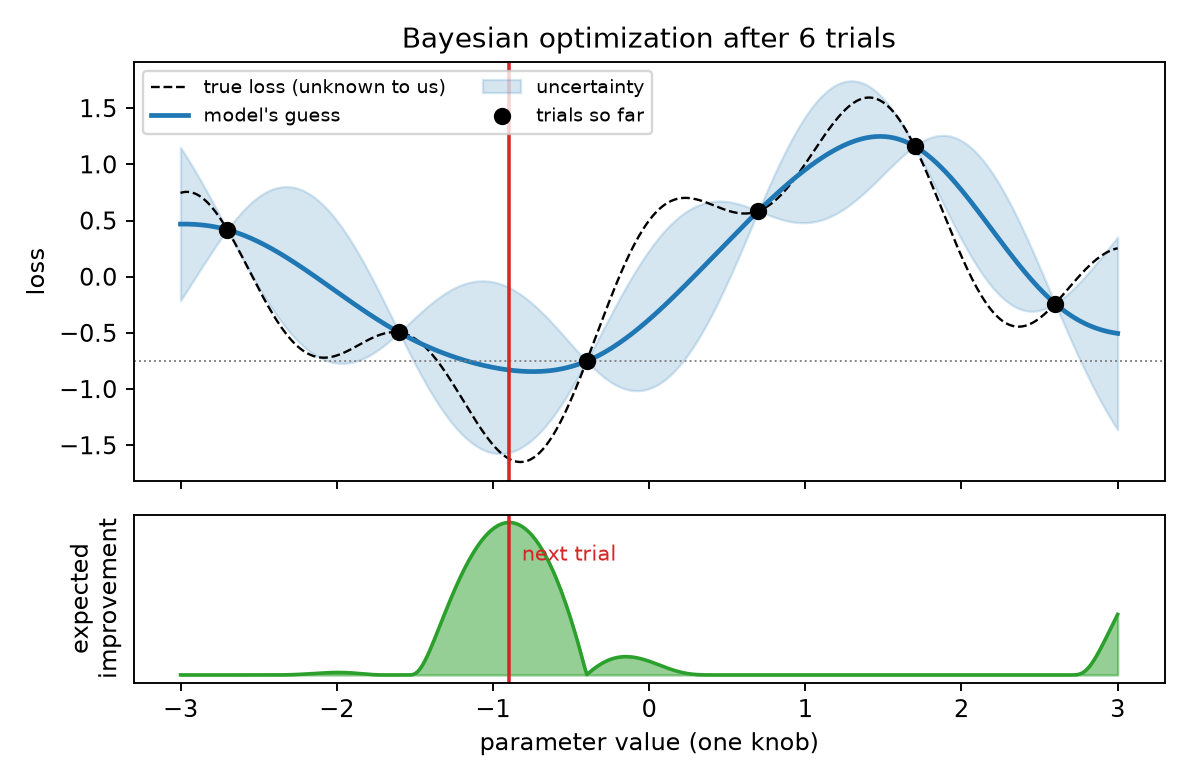
\includegraphics[width=\textwidth]{gp_intuition.png}
    \column{0.47\textwidth}
      \small
      You can only afford a few hundred trials. After each one:
      \begin{enumerate}
        \item Fit a smooth guess through every result so far, \emph{with error bars}.
        \item Try next wherever the guess is low \textbf{or} the error bars are wide.
      \end{enumerate}
      \vspace{0.2em}
      That trade-off has a name, \emph{Expected Improvement}:
      \[ \mathrm{EI} = \underbrace{(\mathcal{L}^* - \mu)\,\Phi(z)}_{\text{probably good}} + \underbrace{\sigma\,\varphi(z)}_{\text{haven't looked}} \]
      \takeaway{Every trial is chosen by the model, not by a fixed rule.}
  \end{columns}
\end{frame}

% 7 ---------------------------------------------------------------------------
\begin{frame}{First attempt: Bayesian optimization on all 24 knobs}
  \begin{columns}[c]
    \column{0.5\textwidth}
      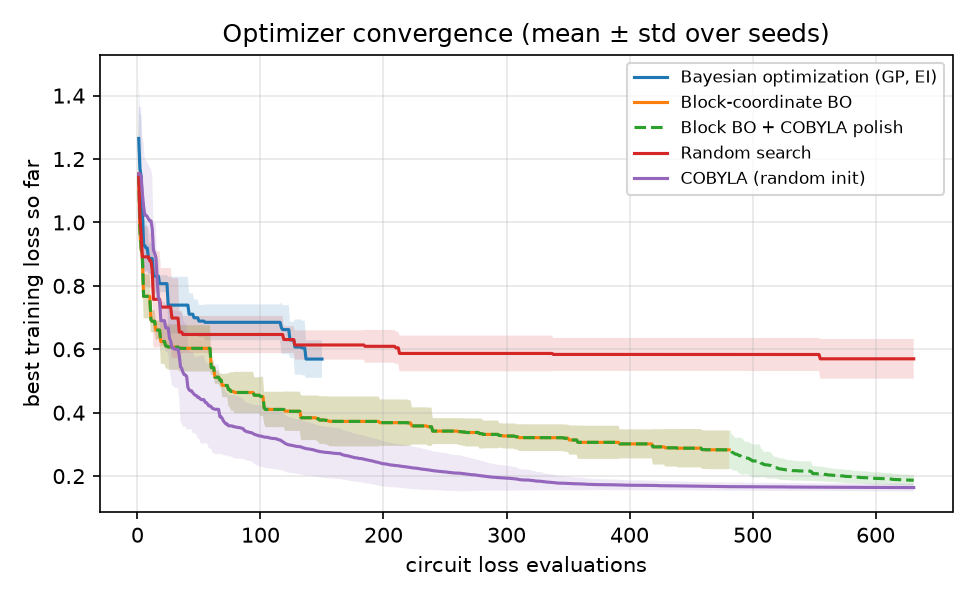
\includegraphics[width=\textwidth]{convergence.png}
    \column{0.48\textwidth}
      \small
      \begin{itemize}
        \item Blue: BO over all 24 knobs at once, 150 trials. Red: 24 knob settings picked \textbf{completely at random}.
      \end{itemize}
      \vspace{0.3em}
      \takeaway{They overlap. Bayesian optimization was no better than guessing. Test accuracy 79\,\% for both.}
      \vspace{0.5em}
      \textbf{Why?} With 24 knobs the space is enormous. 150 trials is far too few for the model to learn its shape, so its guess stays flat and ``try where the error bars are wide'' means ``try anywhere''. More trials and other selection rules did not help.
  \end{columns}
\end{frame}

% 8 ---------------------------------------------------------------------------
\begin{frame}{Fix 1: tune six knobs at a time}
  \small
  \begin{columns}[T]
    \column{0.5\textwidth}
      \textbf{The idea}
      \begin{itemize}
        \item The circuit has four layers of six knobs each.
        \item Freeze three layers. Run Bayesian optimization on the \textbf{six knobs} of the remaining one, 40 trials.
        \item Move to the next layer. Go round all four layers three times.
      \end{itemize}
      \vspace{0.5em}
      \textbf{The analogy}\\
      Tuning a guitar one string at a time, then going round again, instead of turning all six pegs at once.
    \column{0.46\textwidth}
      \textbf{Why it works}
      \begin{itemize}
        \item In six dimensions, 40 trials is enough for the model to actually learn the shape of the landscape.
        \item We only ever accept a change that improves the score, so it can never get worse.
      \end{itemize}
      \vspace{0.5em}
      \takeaway{Same optimizer, same kind of budget: accuracy jumps from 79\,\% to 93\,\%.}
      \vspace{0.2em}
      Still a bit unlucky on some seeds (88 to 97\,\%): it can get stuck where no \emph{single} layer can improve things.
  \end{columns}
\end{frame}

% 9 ---------------------------------------------------------------------------
\begin{frame}{Fix 2: finish with a local ``polish'' (COBYLA)}
  \begin{columns}[T]
    \column{0.5\textwidth}
      \textbf{What COBYLA is}
      \begin{itemize}
        \item A classic optimizer from 1994. \textbf{Not} Bayesian: no model, no error bars.
        \item Looks at the scores of a few nearby knob settings, fits a \emph{flat plane} through them, and steps toward the low side.
        \item If the step helped, take another. If it didn't, take smaller steps.
      \end{itemize}
      \vspace{0.3em}
      \textbf{The analogy}\\
      Walking downhill in fog: feel the slope under your feet, step that way, shorten your stride when you start going up.
    \column{0.46\textwidth}
      \textbf{How we used it}
      \begin{itemize}
        \item Start from the best setting Bayesian optimization found.
        \item 150 small downhill steps.
      \end{itemize}
      \vspace{0.5em}
      \takeaway{Bayesian optimization finds the right valley. COBYLA walks to the bottom of it. Result: 96\,\% on every seed.}
      \vspace{0.3em}
      \small Global search first, local search second. This is a standard pairing.
  \end{columns}
\end{frame}

% 10 --------------------------------------------------------------------------
\begin{frame}{Two sanity checks (the ``controls'')}
  \small
  A result only means something if you know what the dumb alternatives would have scored. Same budget of circuit runs for all.
  \vspace{0.6em}
  \begin{columns}[T]
    \column{0.48\textwidth}
      \textbf{Control 1: random guessing}
      \begin{itemize}
        \item Pick 24 random knob settings, score them, keep the best. Repeat 631 times.
        \item Scored \textbf{79\,\%}.
        \item Tells us whether an optimizer is doing anything at all.
      \end{itemize}
    \column{0.48\textwidth}
      \textbf{Control 2: COBYLA on its own}
      \begin{itemize}
        \item The same downhill walker, but starting from a \emph{random} point, with no Bayesian optimization first.
        \item Scored \textbf{96\,\%}, just like our full pipeline.
        \item Tells us whether the Bayesian part was actually needed.
      \end{itemize}
  \end{columns}
  \vspace{0.8em}
  \takeaway{Control 2 is the uncomfortable one: on our noise-free simulator, the landscape was smooth enough that simply walking downhill from anywhere worked.}
\end{frame}

% 11 --------------------------------------------------------------------------
\begin{frame}{The classical competitors}
  \small
  \begin{columns}[T]
    \column{0.5\textwidth}
      Three models, from simplest to biggest:
      \begin{itemize}
        \item \textbf{A straight line} (3 weights). The baseline that \emph{can't} curve.
        \item \textbf{A tiny neural network} (17 weights). Chosen to match our circuit's 24 knobs as closely as possible. This is the fair fight.
        \item \textbf{A big neural network} (1185 weights). Shows the ceiling when size is no object.
      \end{itemize}
    \column{0.46\textwidth}
      \textbf{How they were trained}
      \begin{itemize}
        \item With gradients, the way neural nets normally are: backpropagation computes the slope of the error for every weight at once.
        \item An optimizer called L-BFGS then follows that slope, using the curvature it picks up along the way to take smart, long steps.
        \item Converges in under a second.
      \end{itemize}
      \vspace{0.2em}
      \takeaway{The classical models get every advantage. Can the gradient-free circuit keep up?}
  \end{columns}
\end{frame}

% 12 --------------------------------------------------------------------------
\begin{frame}{Results}
  \begin{columns}[c]
    \column{0.58\textwidth}
      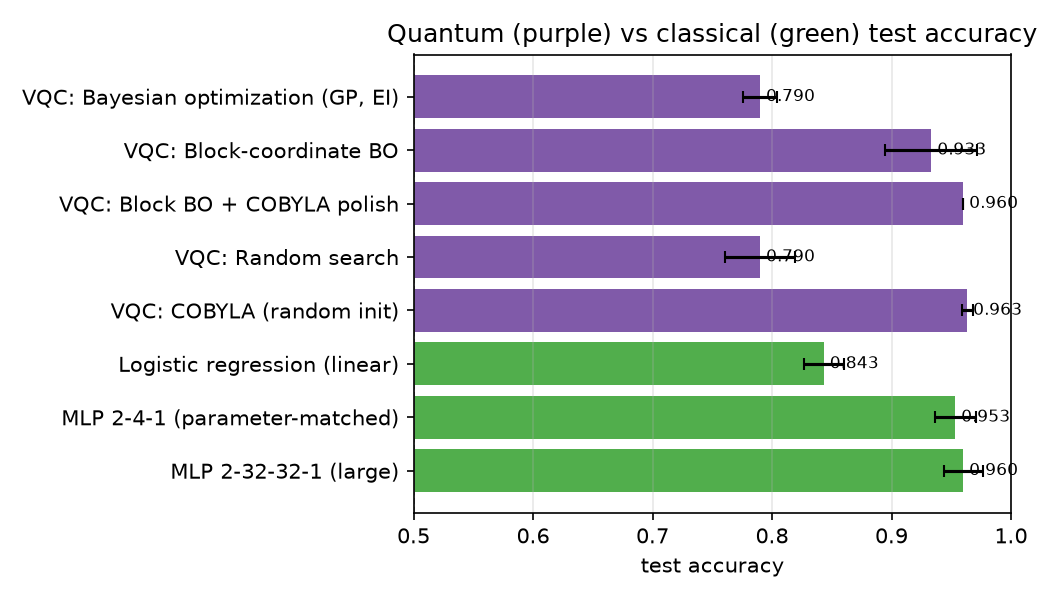
\includegraphics[width=\textwidth]{accuracy.png}
    \column{0.4\textwidth}
      \small
      \begin{enumerate}
        \item \textbf{The quantum circuit reaches 96\,\%}, the same as the neural networks.
        \item BO over all 24 knobs at once was \textbf{no better than random guessing} (79\,\%).
        \item BO on 6 knobs at a time fixed it (93\,\%); the polish made it reliable (96\,\%).
        \item COBYLA alone also reached 96\,\%.
      \end{enumerate}
      \vspace{0.2em}
      \footnotesize 3 random seeds, 100 test points: a one-point gap is noise. Still 95\,\% when read out with only 256 measurement shots per point, as on real hardware.
  \end{columns}
\end{frame}

% 13 --------------------------------------------------------------------------
\begin{frame}{What the models learned}
  \centering
  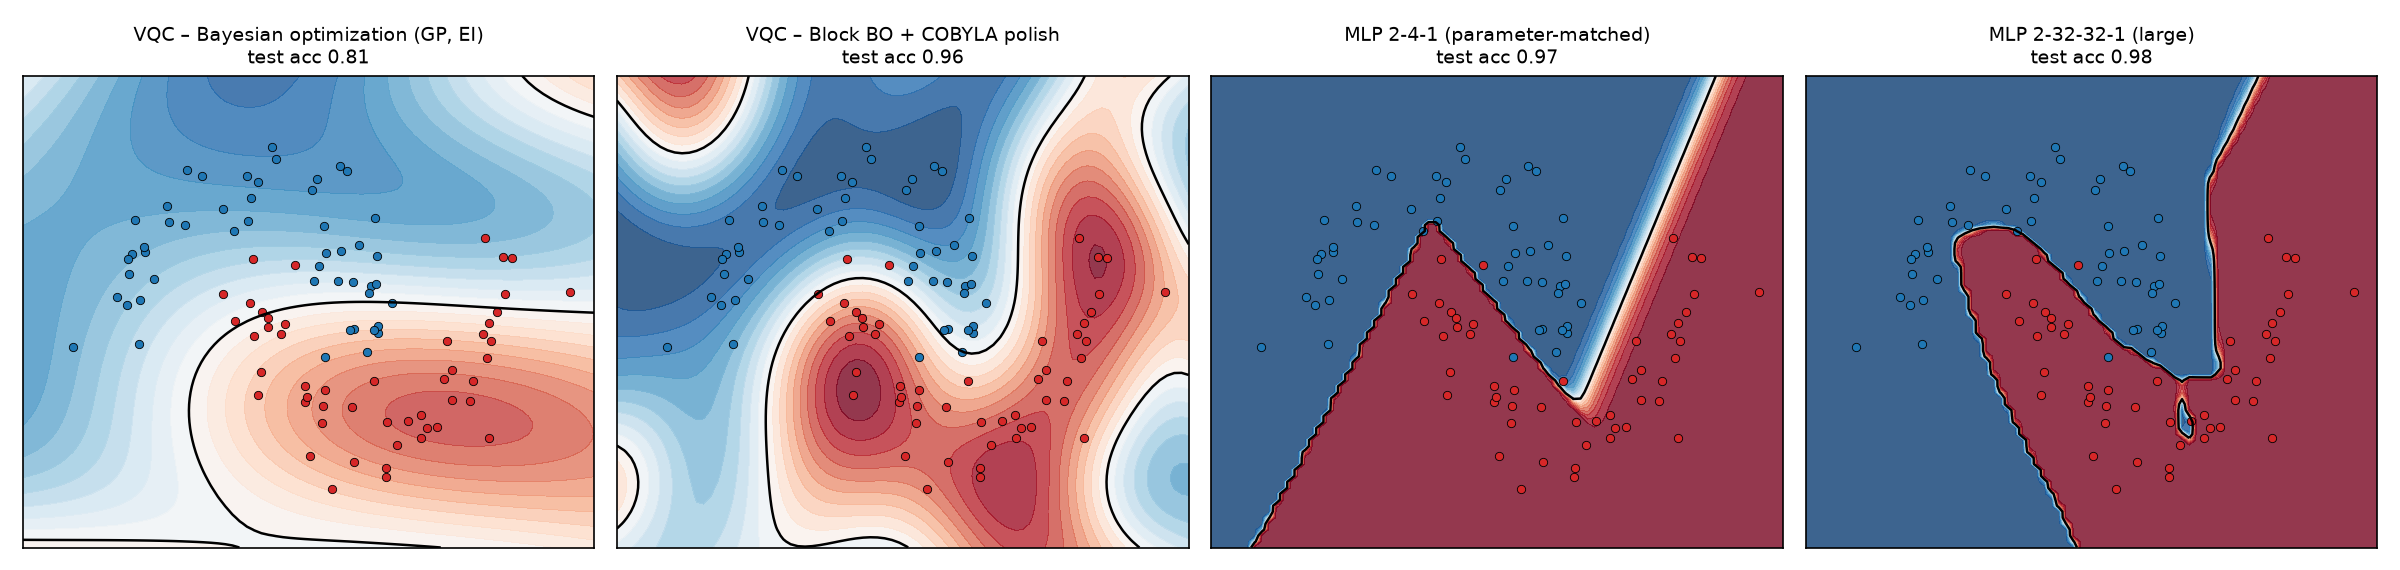
\includegraphics[width=\textwidth]{decision_boundaries.png}
  \vspace{0.4em}
  \begin{columns}[T]
    \column{0.48\textwidth}
      \small Left to right: the boundary goes from a blob (BO on all 24 knobs) to a curve that hugs the moons (BO on 6 at a time + polish).
    \column{0.48\textwidth}
      \small The quantum boundary is \textbf{smooth and wavy}; the neural net's is made of \textbf{straight segments}. Same problem, different shapes.
  \end{columns}
\end{frame}

% 14 --------------------------------------------------------------------------
\begin{frame}{Conclusions}
  \begin{enumerate}
    \item A 2-qubit circuit with 24 knobs, trained with \textbf{no gradients at all}, matched classical neural networks with 17 and 1185 weights: 96\,\% on every seed.
    \vspace{0.3em}
    \item Bayesian optimization \textbf{cannot handle all 24 knobs at once}. It only works when restricted to a handful of knobs at a time, and a short local polish makes it reliable.
    \vspace{0.3em}
    \item On a noise-free simulator, the simpler downhill walker COBYLA did just as well on its own. Bayesian optimization's real advantages are in noisy, expensive-to-evaluate settings, which our simulator does not create.
    \vspace{0.3em}
    \item The trained circuit survives realistic measurement: 95\,\% with 256 shots per point.
  \end{enumerate}
  \vspace{0.6em}
  \takeaway{Not a quantum advantage, and none expected at 2 qubits. The point was showing which training methods work when gradients are off the table.}
  \vspace{0.4em}
  \begin{flushright}\footnotesize Code, results and a live terminal demo: \texttt{bo-vqc} repository\end{flushright}
\end{frame}

\end{document}
